\documentclass[a4paper]{article}
\usepackage{times}
\usepackage{hyperref}
\usepackage{graphicx}
\usepackage{amssymb}

\title{{\bf Architecture} \\
  for the UML Reference Animator}
\author{Greg O'Keefe}
\begin{document}
\maketitle 


We describe how the UML Reference Animator will work.  This is the
very big picture, and is a work-in-progress.  The aim is to guide and
encourage further discussion toward a clear and common understanding
of what we are building.  In addition to the proposed shape of the
working product, we describe the current status of prototype
development and investigation.

We take a ``functional'' perspective on the proposed system, that is,
we focus on the datatypes and the transformations on these types.
Important aspects such as user interface and module or package
structure will need to be addressed elsewhere.

The functional architecture is indicated in Figure \ref{figArch}.
(Sorry about the wierd arrows {\sf editor} and {\sf transitioner}.)
The following Section explains this diagram, discussing each of the
diagram elements in turn.  Section \ref{prototyping} presents what we
know and what we can currently do with respect to each of these
elements.  The path from this current situation to a completed working
product is outlined in Section \ref{roadmap}.

\begin{figure}
\begin{center}
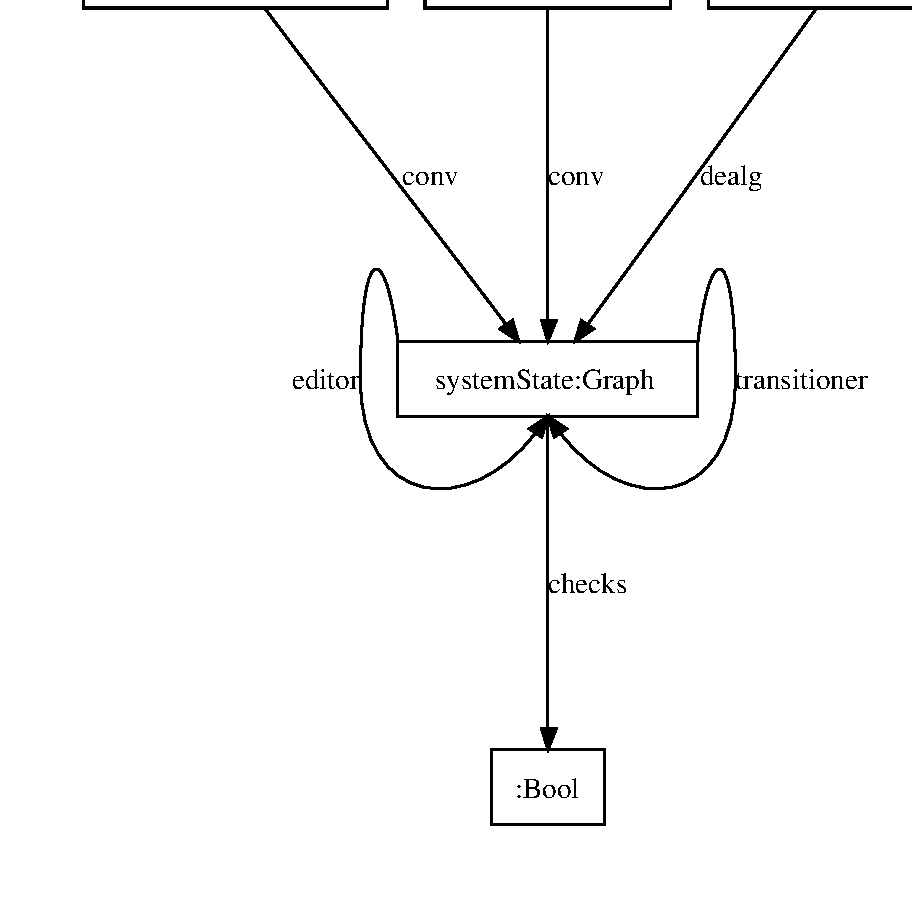
\includegraphics{architectureFig.ps}
\end{center}
\caption{Functional architecture}
\label{figArch}
\end{figure}

\section{Architecture}
The animator will make UML's semantics concrete by enabling system
states to be built for a given UML model, and these states to evolve,
creating execution traces for the model.

The central role of UML system states is indicated their position in
Figure \ref{figArch}.  Following our thesis \cite{myThesis}, UML
system states are graphs, and contain the model, and the metamodel
etc.  

Like practically all modern UML modelling tools, we will be working
with UML models as stored in the UML implementation in the Eclipse
Modelling Framework (EMF).  Converting such a model into a graph
should be a very straightforward model transformation from the UML
metamodel to a Graph metamodel.  This model transformation is
indicated in Figure \ref{figArch} by the edges labelled {\sf conv}.
UML models in the UML/EMF repository do \emph{not} include the
metamodel, which to satisfy parts of the UML definition, they really
should.  We will rectify this by adding the UML metamodel to the
system state graphs.  Since the UML metamodel is a UML model, the same
model transformation {\sf conv} can be used for this task.

In addition to the model and the metamodel, a system state will
typically have objects, event occurrences and behavior executions.
The objects are most naturally described by an object diagram.  The
object icons in object diagrams actually represent
InstanceSpecifications rather than objects, and this is how graphical
object diagram editors will store them.  But it does make sense to
interpret them as objects, and to allow users to use whatever object
diagram editing tools they prefer.  We will therefore require a model
transformation that performs this ``reinterpretation''.  It turns out
that the InstanceSpecification form of an object diagram is really
just the ``algebraic'' form of the collection of objects and links we
would normally associate with it \cite{myThesis}.  The model
transformation is therefore called {\sf dealg} which is short for
``dealgebrisation''.  

Thus, given a Graph metamodel and these two (hopefully simple) model
transformations, we can obtain system states as graphs, but these
system states may be incomplete in some ways.  Such a system state
would not have any event occurrences.  When constructing an initial
state for an example trace, modellers usually presume the system is
quiescent, in the sense that no objects have event occurrences in
their event pools waiting to be actioned.  Behavior executions for the
classifier behaviors of active objects might be produced by the {\sf
  dealg} transformation.  Since Behavior is a Classifier, one could
describe them using an InstanceSpecification. A bit of research in
\cite{UML22super} is required to determine whether the current state
can be specified when such a behavior execution is an instance of a
state machine.

It seems likely that not all of a system state can be fully specified
by UML model elements.  We will almost certainly require the ability
to directly edit the system state.  It is especially important to
consider the interface here, because the point of the animator is to
enable the modeller to see and construct all the possibilities
described by their model.  The system states are the static
possibilities, and the system state transitions determine the dynamic
possibilities.  Whatever form this system state edit facility takes,
from a functional point of view, it takes system states and returns
system states.  It is shown in Figure \ref{figArch} as the edge {\sf
  editor}.

The dynamic semantics of UML is the transitions that are possible
between system states.  Our project, following \cite{myThesis} assumes
that these transition possibilities are expressed as a fixed set of
graph transformation rules.  These rules and the facilities needed to
apply them to a system state to obtain the resulting system state are
shown in Figure \ref{figArch} as the {\sf transitioner} arrow.  Again,
it is cruicial that this is presented in an easily useable way, but
from a functional point of view, we require that all and only legal
UML system state transitions can be performed.

A UML model contains both prescriptive and descriptive parts.  Classes
say what kinds of objects can exist, and are therefore prescriptive.
OCL constraints on the other hand describe a condition that might or
might not be true in a given system state, although, we usually state
them because we want them to be true!  Similarly, sequence diagrams
can not determine what happens in a system execution because this is
determined by the defined behaviors of the objects.  The sequence
diagram just tells a story that we hope can, or will happen.  The {\sf
  check} arrow stands for ways of evaluating these descriptions on a
given system state.

So, given a UML model, we have the means to create system states for
it in graph from.  These system states contain their model and the
metamodel.  We can modify the system states as needed, and we can
evolve them according to the execution rules of UML.  Finally, we can
evaluate various descriptions on system states.

\section{Prototyping}
\label{prototyping}

This section roughly describes bits and pieces of work towards the
achitecture elements described above.  The purpose is to hand the work
over to the whole team so we can make more progress.  The plan is to
\emph{show} each of the things discussed here during our session on
Tuesday 12 May 2009.

\subsection{UML and its Metamodel}
The UML/EMF datatype is provided by the Eclipse plugins, along with
lots of editors, code, code generation facilities etc etc.

The UML metamodel is available from the OMG website as a small
collection of {\tt .xmi} files.  Since the UML metamodel is a UML
model, these can be read in using the UML/EMF plugins in Eclipse,
which shows the metamodel as a great big tree.

UML models can be created using the UML/EMF plugins, or graphical
editors built on top of this.  This is what modellers do!  

\subsection{Graphs in Eclipse}
We have a simple Ecore metamodel for list-graphs, which may need
rethinking.  It is presently in Greg's Eclipse workspace, project
ListGraph.  The Ecore diagram editor was used to create it, but the
diagram and model seem to be out of synch now.  An editor has been
generated for this metamodel, which could serve as a prototype for the
{\sf editor} in Figure \ref{figArch}.

\subsection{Model Transformations}
There are many model tranformation languages available, but Greg has
some familiarity with Kermeta.  This is a simple java-like language
with the ability to work with models in Eclipse.  The ListGraph
project in Greg's Eclipse workspace contains a Kermeta program which
reads a graph model and generates a {\tt .dot} file from it, so that
the dot program can be used to see it.

\subsection{Graphs in Haskell}
The Eclipse/Java environment provides nice user interface and
integration capabilities, but it is pretty cumbersome for prototyping
mathematical ideas.  Therefore the majority of the prototyping work
has been done using Haskell.  This work is described in detail in a
separate document, \emph{List-Graphs: Theory and Implementation}.


\section{Development Roadmap}
\label{roadmap}
This section needs to be written.  It will describe the work and
milestones which will lead us to a working, authoritative and useable
UML animator.

\bibliographystyle{alpha} 
\bibliography{../../Research/bibtex}

\end{document}

